%===================================== CHAP 2 =================================

\chapter{Background Theory}

\section{Artificial Neural Networks}

\textit{This was missing in the specialization project. Need to cover all concepts used later in the report. This includes all different layers of a neural network. The layers (dropout, pooling, etc) could perhaps be a separate section after this one.}

\subsection{Basics}

\subsubsection{The Neuron}

Artificial Neural Networks (ANNs) are inspired by the structure and behavior of a biological brain, but they are generally not intended to be realistic models. A neural network consist of interconnected nodes referred to as units. These correspond to a biological neuron, the basic computational unit of the brain, structured as illustrated in \textbf{Fig. \ref{fig1}}. The connections between the units in an  corresponds to a biological neuron's dendrites, which provide input signals, and its single axon, which produces output signals and is connected to other neurons. \\

\begin{figure}
    \begin{minipage}{0.5\textwidth}
        \centering
            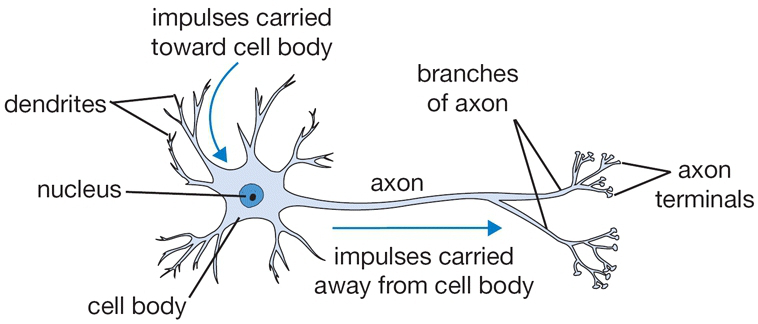
\includegraphics[width=1\textwidth]{fig/neuron}
            \caption{Biological neuron\cite{cs231n_part1}}
            \label{fig1}
    \end{minipage}
    \begin{minipage}{0.4\textwidth}
        \centering
            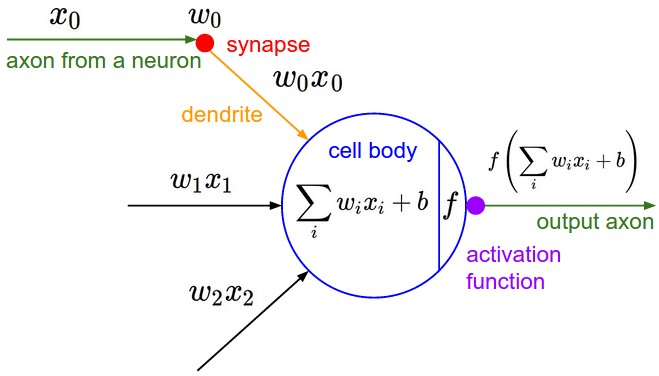
\includegraphics[width=1\textwidth]{fig/neuron_model}
            \caption{Mathematical model of a neuron\cite{cs231n_part1}}
            \label{fig2}
    \end{minipage}
\end{figure}

\noindent To simulate these signals, an ANN uses a mathematical model as illustrated in \textbf{Fig. \ref{fig2}}, where the signal is multiplied by the weight of a connection. The weight of a specific connection control how much the unit on one end influences the unit on the other end. The sum of all input signals are computed at the cell body of the unit. If this sum is above a certain threshold, the unit fires an output signal determined by its activation function by performing a specific mathematical operation on the sum.

\subsubsection{Organization}

\noindent The idea of an ANN is that it can approximate any continuous function, and that it has the possibility of learning. The simplest form of an ANN is the single layer perceptron, which consists of only one layer of output nodes. This network can only learn linearly separable patterns. To allow for learning complex patterns, more layers need to be added. As layers are added, the depth of the network increases. This is why we refer to the the use of multi-layer perceptrons (MLPs) as "deep learning". \\

\noindent There are several different classes and types of ANNs. We will only describe the feedforward neural network, which is the original version, and thus we will use the term ANN when referring to such a network. In this kind of network, all connections are directed from one layer to the next layer, and there are no cycles or connections between units in the same layer. A network with cycles is called a recurrent neural network (RNN).

\subsection{The Learning Process}

The weights of a model can be learned by training the model on a set of input and output values, a task which is called supervised learning. There are also other kinds of learning, but we will not cover these. The learning process runs for a number of epochs, meaning the number of times the learning algorithm will see the entire data set. Often, the data is split into so-called batches when passed to the algorithm. The batch size is thus the number of training examples in a batch.

\subsubsection{Loss Function}

\noindent The goal of an ANN is to find a function that solves a certain problem, more specifically that finds an optimal solution to the problem. The definition of this optimal solution is that given a loss function, there are no other solution with less of a loss. The loss function is in that sense a measure of how far away a solution is from an optimal solution. The goal of the learning process is thus to find a function with the smallest possible loss. The weights of a model can be learned by training the model on a set of input and output values, a task which is called supervised learning. There are also other kinds of learning, but we will not cover these. In supervised learning, the goal is to find the function that best maps the input to the output. The loss will then be the mismatch between such a mapping and the example data. \\ 

\subsubsection{Gradient Descent}

\noindent To optimize the loss, we can use an algorithm called gradient descent, which minimizes any function iteratively. The process is a repeated loop of evaluating the gradient of the loss function, and then updating the weights based on this gradient. There are a number of different algorithms to optimize this process, and we will briefly describe the ones commonly used in a later section. The simplest form of this algorithm, also called its vanilla version, looks something like this: \\

\begin{lstlisting}
    for i in range(epochs):
        weights_grad = evaluate_gradient(loss_function, data, weights)
        weights += - learning rate * weights_grad
\end{lstlisting}

\noindent First, the algorithm evaluates the gradient of the loss function for the whole data set with respect to the current weights. Then it updates the weights based on the evaluated gradient and a learning rate. The learning rate controls the magnitude of the update, and is a crucial network hyperparameter setting. This process is repeated for a pre-defined number of epochs.

\subsubsection{Backpropagation}

\noindent Backpropagation is an algorithm for computing the gradients in combination with gradient descent.

Backpropagation is an algorithm that is used in combination with gradient descent. 

\noindent Describe backpropagation.

\subsection{The Activation Function}

\noindent There are a great variety of activation functions in use, but we will only briefly describe those most commonly used and thus considered in our implementation. The mathematical function of these are plotted in \textbf{Fig. \ref{activationfuncs}}. For further details we refer the reader to the Stanford CS class on convolutional neural networks\cite{cs231n_part1}. The common behaviour of all activation functions is that they define the output of a unit given a set of inputs. \\
\begin{figure}[H]
    \begin{minipage}{0.3\textwidth}
        \begin{tikzpicture}
            \begin{axis}[
                title = {Sigmoid function},
                axis lines = center,
                xtick={-10, -5, 5, 10},
                ytick={0, 0.2, 0.4, 0.6, 0.8, 1.0},
            ]
            \addplot [
                domain=-10:10,
                samples=100,
                color=blue,
            ]
            {1 / (1 + e^-x)};
            \end{axis}
        \end{tikzpicture}
    \end{minipage}
    \begin{minipage}{0.3\textwidth}
        \begin{tikzpicture}
            \begin{axis}[
                title = {Tanh function},
                axis lines = center,
                xtick={-10, -5, 5, 10},
                ytick={-1.0, -0.5, 0, 0.5, 1.0},
            ]
            \addplot [
                domain=-10:10,
                samples=100,
                color=blue,
            ]
            {(2 * (1 / (1 + e^-(2*x)))) - 1};
            \end{axis}
        \end{tikzpicture}
    \end{minipage}
    \begin{minipage}{0.3\textwidth}
        \begin{tikzpicture}
            \begin{axis}[
                title = {ReLU function},
                axis lines = center,
                xtick={-10, -5, 5, 10},
                ytick={2, 4, 6, 8, 1.0},
            ]
            \addplot [
                domain=-10:10,
                samples=100,
                color=blue,
            ]
            {max(0, x)};
            \end{axis}
        \end{tikzpicture}
    \end{minipage}
    \caption{The most commonly used activation functions}
    \label{activationfuncs}
\end{figure}

\subsubsection{Sigmoid}

The sigmoid activation function is mathematically defined as $\sigma(x) = 1/(1 + e^{-x})$. The function takes a number as input, and outputs a number within a continuous range from 0 to 1. The sigmoid function has previously been used a lot, but because of its drawbacks, other activations functions tend to be preferred nowadays. The first drawback is that the outputs are not centered around zero, which can cause undesirable behaviour during gradient descent. A bigger drawback is that the activation saturates, meaning that the unit outputs mostly 0 and 1 instead of anything in between, and thus the gradient at these regions is very low. If the gradient falls to zero, the weights will not be updated through gradient descent, and so the network will stop learning.

\subsubsection{Tanh}

The tanh activation function is a scaled version of the sigmoid function. Its mathematical function is $tanh(x) = 2\sigma(2x) - 1$. The scaling causes the tanh function to output numbers within the range of -1 and 1. This makes the output zero-centered, thus avoiding the first drawback of the sigmoid function. Even though the tanh function still stuffers from saturation, it is preferred to the sigmoid function.

\subsubsection{ReLU}

The Rectified Linear Unit (ReLU) activation has the mathematical function $f(x) = max(0,x)$. This means that it is very close to linear; thresholding the input at zero, but keeping any value above. It has become very popular, and is in general the activation function of choice. It is non-saturating, and has been found to speed up the convergence of stochastic gradient descent. The computation of the function is also very inexpensive compared to the sigmoid and tanh function. The only problem with the ReLU function is the possibility of "dead" units, meaning that they will never activate. Generally, lowering the learning rate can prevent this, but there have also been several attempts to fix this issue, for instance using so called PReLU or Maxout units.

\subsection{Optimization}

\subsubsection{Stochastic Gradient Descent}

The vanilla version of gradient descent is also called batch gradient descent. A batch of data is a portion of the training data, in this case the entire training data set. The gradient is computed over such a batch, which is very slow and expensive in terms of memory. \\

\noindent Stochastic gradient descent (SGD) improves the vanilla version. In this case, the gradient is computed over mini-batches consisting of only one training pair. This is a special case of the more general mini-batch gradient descent, which computes the gradient over batches of the training data, instead of the entire set. SGD refers to both mini-batch gradient descent, as well as the special case of stochastic gradient descent. Usually it is more efficient to compute the gradient over a number of examples instead of only one. Even though SGD is much more efficient than the vanilla version, it also has its drawbacks, and therefore a number of algorithms intended to improve this has been developed.

\subsubsection{Momentum}

One way to improve SGD is to add momentum. SGD can get stuck in local optima, and adding momentum can help accelerating in the right direction. A further improvement is the Nesterov momentum, which adds some notion of where SGD is heading by approximating the next position.

\subsubsection{Adaptive Learning Rate Methods}

Adaptive learning rate methods are algorithms that automatically adapts the learning rate to the parameters. They are quite similar, and perform thereafter. In general, SGD often finds a minimum, but these methods can help to achieve faster convergence, and you do not have to tune the learning rate. The algorithms are usually implemented with a good default starting value. \\

\noindent Adagrad was the first adaptive learning rate method proposed, and the others are thus extensions to this. Its weakness is that the learning rate decreases and eventually becomes close to zero. Adadelta and RMSprop are methods that try to overcome this, and they are close to identical. Adam adds some form of momentum to the optimization, and might be the best overall choice.


\begin{itemize}
    \item backpropagation
\end{itemize}

\subsection{Architecture}

\begin{itemize}
    \item Input and output layers
    \item Fully-connected layer
    \item Hidden layers
    \item Deep models
    \item Convolutional layer
    \item Dropout layer
    \item Pooling
\end{itemize}

\section{Convolutional Networks}

\textit{More in-depth than covered in the specialization project. \\
What exactly is the convolutional operation? Convolutional layer (local connections and weight sharing) vs normal layer.}

\section{Residual Networks}

\section{Face Recognition}

\textit{Can probably use a lot from the specialization project here.}

\section{Facial Expression}

\textit{Here as well.}

\section{Visualization}
\textit{Describe all the different techniques, perhaps in more detail. \\
Possibly even implementation level.}

\subsection{Why Visualize?}

When using ANNs to solve complex problems, like face recognition, it is not unlikely that the network requires millions of parameter values to obtain a desirable performance level. In these cases, it is hard to gain insight about the network's performance by examining the parameter values directly, both because of the unfeasible amount of values and each value's relative insignificance. However, when applying ANNs to tasks in the image domain, there are several ways to help us understand the inner workings of the network by presenting information in the same readable format as the input. Aside from the fact that images more suited than numbers for human readability, there exists several techniques that utilizes the connections in the network to produce visualizations. These images can then provide insight into a larger part of the network, spanning several layers, possibly the whole network. Through the use of these visualization techniques, the network can improved by making informed decisions, instead of employing a trial and error approach.

\textit{Visualization offers a reasonable method for presenting the vast amount of information available when analyzing a convolutional neural network in a readable manner. For example, one technique allows us to view which areas of an input image a classifying network focuses on, informing us on what the network discerns as important when computing output classifications}. \\

\noindent \textit{To gain a beneficial amount of information from our visualization website, we determined several different techniques to be researched. In this section, we present the techniques we have selected as appropriate for our purpose. Their advantages and relevance are discussed, and a brief description of how they function are given. For further explanations on implementation, we refer the reader to their respective articles.} 

\subsection{Training Progress Measurements}

Throughout training, the progress of the network is visualized in a simple line plot. Measurements are made of the standard network appraisal values, loss and accuracy, both on the training set data and, if provided, the validation set data. A typical thing to want to monitor, these values provide a means to explicitly evaluate a network’s performance. Plotting these values against time, at certain batch intervals or at epoch completion, puts the current measurements in perspective, and makes the training progress, or lack thereof, easily discernible. The shape of the line plot could also be used to reveal undesirable values in the training hyperparameters. For example, if the learning rate is too large, the network is likely to vastly improve at first, only to have its progress quickly stagnate. In this case, both loss and accuracy plots would have distinct shapes that indicate a problem, without having to look at any of their actual values.

By including the validation values, one could also be able to identify the presence of overfitting, marked by a point where the validation accuracy begins to decline while training accuracy continues to rise.

\textit{The training progress measurements include standard network appraisal values, like loss and accuracy on the training set data, and the loss and accuracy of the validation set data, if provided. It is a typical thing to monitor, and provides a means to explicitly evaluate a network’s performance. Plotting these values against time, for example at each batch or epoch completion, puts the current measurements in perspective, and makes the training progress, or lack thereof, easily discernible. By including the validation values, one could also be able to identify the presence of overfitting, marked by a point where the validation accuracy begins to decline while training accuracy continues to rise.}

\subsection{Layer Activations}

\textit{The activation output is most readable for the convolutional layers, and especially so for the earlier ones. The activations in convolutional layers can also be called feature maps, and the units in these maps typically share the same weight matrix, called the filter. The filter will, through backpropagation, learn to look for certain features, for example a horizontal edge. Applying the filter to the input creates the feature map, which can convey information about where the filter found the feature it was looking for. For deeper convolutional layers, these features become more complex and so does the input. It is the simplicity of their filters and input that make the earlier layers activations easier to interpret. Considering these filters, the activation output can be helpful to confirm that the network is progressing well, if the output is showing signs of activation in areas with similar features. These patterns should become more and more clear as training goes on, and when the activations start experiencing little or no change, the proper filters should be obtained.} \\

\noindent \textit{Additionally, in networks using ReLUs, a common activation function, the expectation of seeing sparse and localized activations can be confirmed, which is an indicator of the network learning properly. If some feature maps are entirely dark, with all pixel values zero, this can be a warning sign that the learning rate is too high. The particular filters are then rendered useless, and they have no possible way to recover \cite{cs231n_act}. }

\subsection{Salience Maps}

\textit{A salience map is typically a black-and-white image with the same size as the input, where important pixels have a high value, and insignificant pixels have a low value \cite{salience}. Thus, the important regions can be easily identified by their brightness. A map for classification is specific to an image and a class, and it allows us to observe which parts of an image influences the network classification score the most. In other words, we can view which parts of an image that the network deems more important when deciding upon the classification score chosen. Such a map can be produced by efficiently using the back-propagation gradient of the output score with respect to the input image.} \\

\noindent \textit{In a face recognition case, the saliency would allow us to investigate what the network emphasizes, for example which facial regions are decisive in producing the identification output. We could also exploit salience maps for expression classification, creating maps to display which areas were the most influential for selecting the outputted expression results. By using the insight gained through salience maps, we would be able to confirm our beliefs that a network focuses on regions containing important feature information, and alert us to any peculiarities.}

\subsection{Deconvolution}

\textit{Deconvolution involves using a deconvolutional network, which can be thought of as a reverse convolutional network \cite{deconv_net}. The aim of visualizing deconvolution is to map the feature activity present in the intermediate layers back to the input pixel space \cite{deconv_vis}. This enables us to see what the input pattern that caused the activation looks like. To acquire the pattern for a certain activation, we first feed an image into the regular network to get the activations, then set all the the other activations in the relevant layer to zero, and finally feed these feature maps into the appropriate layer in the deconvolutional network.} \\

\noindent \textit{By identifying the input patterns responsible for the activations, we should be able to understand what each feature map is concentrated on. This could help explain why we experience similar activations on images that are seemingly unrelated, if the feature map is focused on something unexpected, like an object in the background. It also demonstrates the hierarchy among the maps, as deconvolution for later layers will reveal more complex patterns.} \\

\noindent \textit{Viewing the progression of these patterns during training can tell us something about their development. The patterns of the lower layers will typically converge early, possibly after a few epochs, while the complex layers further up will have slower converging patterns, maintaining the need for substantial network training. If any patterns have trouble converging, it could signal a potential problem with the model.}

\subsection{Deep Visualization}

\textit{Deep visualization offers visualization of the learned features of a network, computed by the individual neuron at each layer \cite{deepvis, deepvis_web}. The outputs are images that maximally activate individual neurons, and represent what the neurons in the network have learned to look for. Starting with random images, the method iteratively updates the images based on the gradient update of a chosen neuron to create images that optimally triggers the activation of that neuron. For example, in an image classification network, we could use the output neuron responsible for the class ‘cat’, and produce deep visualizations for this neuron. The resulting images should display various catlike features across their pixel space. As we start with random images, the optimization is stochastic, meaning that the variance of these images provides information about the network unit’s learned invariances. In our case, we could choose neurons that classify the face recognition result to similar effect. If the neurons are looking for sensible features, the network is heading in the right direction. If the features portrayed are irrational or intangible, the opposite might be the case.} \\ 

\noindent \textit{The visualization is not restricted to the output units, and can be performed for all neurons in the network. We can then determine what a hidden unit has learned to look for, which would typically be a lower level feature. For very low layers, this could for example be edges. In the face recognition domain, at an intermediate layer, we might get output images depicting an eye, or eyelike features.} \\

\noindent \textit{It is important to note that the technique is reliant on heavy regularization to produce recognizable and interpretable output images.}

\cleardoublepage